%% bare_conf.tex
%% V1.4a
%% 2014/09/17
%% by Michael Shell
%% See:
%% http://www.michaelshell.org/
%% for current contact information.
%%
%% This is a skeleton file demonstrating the use of IEEEtran.cls
%% (requires IEEEtran.cls version 1.8a or later) with an IEEE
%% conference paper.
%%
%% Support sites:
%% http://www.michaelshell.org/tex/ieeetran/
%% http://www.ctan.org/tex-archive/macros/latex/contrib/IEEEtran/
%% and
%% http://www.ieee.org/

%%*************************************************************************
%% Legal Notice:
%% This code is offered as-is without any warranty either expressed or
%% implied; without even the implied warranty of MERCHANTABILITY or
%% FITNESS FOR A PARTICULAR PURPOSE! 
%% User assumes all risk.
%% In no event shall IEEE or any contributor to this code be liable for
%% any damages or losses, including, but not limited to, incidental,
%% consequential, or any other damages, resulting from the use or misuse
%% of any information contained here.
%%
%% All comments are the opinions of their respective authors and are not
%% necessarily endorsed by the IEEE.
%%
%% This work is distributed under the LaTeX Project Public License (LPPL)
%% ( http://www.latex-project.org/ ) version 1.3, and may be freely used,
%% distributed and modified. A copy of the LPPL, version 1.3, is included
%% in the base LaTeX documentation of all distributions of LaTeX released
%% 2003/12/01 or later.
%% Retain all contribution notices and credits.
%% ** Modified files should be clearly indicated as such, including  **
%% ** renaming them and changing author support contact information. **
%%
%% File list of work: IEEEtran.cls, IEEEtran_HOWTO.pdf, bare_adv.tex,
%%                    bare_conf.tex, bare_jrnl.tex, bare_conf_compsoc.tex,
%%                    bare_jrnl_compsoc.tex, bare_jrnl_transmag.tex
%%*************************************************************************


% *** Authors should verify (and, if needed, correct) their LaTeX system  ***
% *** with the testflow diagnostic prior to trusting their LaTeX platform ***
% *** with production work. IEEE's font choices and paper sizes can       ***
% *** trigger bugs that do not appear when using other class files.       ***                          ***
% The testflow support page is at:
% http://www.michaelshell.org/tex/testflow/



\documentclass[conference]{IEEEtran}
% Some Computer Society conferences also require the compsoc mode option,
% but others use the standard conference format.
%
% If IEEEtran.cls has not been installed into the LaTeX system files,
% manually specify the path to it like:
% \documentclass[conference]{../sty/IEEEtran}





% Some very useful LaTeX packages include:
% (uncomment the ones you want to load)


% *** MISC UTILITY PACKAGES ***
%
%\usepackage{ifpdf}
% Heiko Oberdiek's ifpdf.sty is very useful if you need conditional
% compilation based on whether the output is pdf or dvi.
% usage:
% \ifpdf
%   % pdf code
% \else
%   % dvi code
% \fi
% The latest version of ifpdf.sty can be obtained from:
% http://www.ctan.org/tex-archive/macros/latex/contrib/oberdiek/
% Also, note that IEEEtran.cls V1.7 and later provides a builtin
% \ifCLASSINFOpdf conditional that works the same way.
% When switching from latex to pdflatex and vice-versa, the compiler may
% have to be run twice to clear warning/error messages.






% *** CITATION PACKAGES ***
%
%\usepackage{cite}
% cite.sty was written by Donald Arseneau
% V1.6 and later of IEEEtran pre-defines the format of the cite.sty package
% \cite{} output to follow that of IEEE. Loading the cite package will
% result in citation numbers being automatically sorted and properly
% "compressed/ranged". e.g., [1], [9], [2], [7], [5], [6] without using
% cite.sty will become [1], [2], [5]--[7], [9] using cite.sty. cite.sty's
% \cite will automatically add leading space, if needed. Use cite.sty's
% noadjust option (cite.sty V3.8 and later) if you want to turn this off
% such as if a citation ever needs to be enclosed in parenthesis.
% cite.sty is already installed on most LaTeX systems. Be sure and use
% version 5.0 (2009-03-20) and later if using hyperref.sty.
% The latest version can be obtained at:
% http://www.ctan.org/tex-archive/macros/latex/contrib/cite/
% The documentation is contained in the cite.sty file itself.






% *** GRAPHICS RELATED PACKAGES ***
%
\ifCLASSINFOpdf
  \usepackage[pdftex]{graphicx}
  % declare the path(s) where your graphic files are
  \graphicspath{{figs/}}
  % and their extensions so you won't have to specify these with
  % every instance of \includegraphics
  \DeclareGraphicsExtensions{.pdf,.jpeg,.png}
\else
  % or other class option (dvipsone, dvipdf, if not using dvips). graphicx
  % will default to the driver specified in the system graphics.cfg if no
  % driver is specified.
  \usepackage[dvips]{graphicx}
  % declare the path(s) where your graphic files are
  \graphicspath{{../eps/}}
  % and their extensions so you won't have to specify these with
  % every instance of \includegraphics
  \DeclareGraphicsExtensions{.eps}
\fi
% graphicx was written by David Carlisle and Sebastian Rahtz. It is
% required if you want graphics, photos, etc. graphicx.sty is already
% installed on most LaTeX systems. The latest version and documentation
% can be obtained at: 
% http://www.ctan.org/tex-archive/macros/latex/required/graphics/
% Another good source of documentation is "Using Imported Graphics in
% LaTeX2e" by Keith Reckdahl which can be found at:
% http://www.ctan.org/tex-archive/info/epslatex/
%
% latex, and pdflatex in dvi mode, support graphics in encapsulated
% postscript (.eps) format. pdflatex in pdf mode supports graphics
% in .pdf, .jpeg, .png and .mps (metapost) formats. Users should ensure
% that all non-photo figures use a vector format (.eps, .pdf, .mps) and
% not a bitmapped formats (.jpeg, .png). IEEE frowns on bitmapped formats
% which can result in "jaggedy"/blurry rendering of lines and letters as
% well as large increases in file sizes.
%
% You can find documentation about the pdfTeX application at:
% http://www.tug.org/applications/pdftex





% *** MATH PACKAGES ***
%
%\usepackage[cmex10]{amsmath}
% A popular package from the American Mathematical Society that provides
% many useful and powerful commands for dealing with mathematics. If using
% it, be sure to load this package with the cmex10 option to ensure that
% only type 1 fonts will utilized at all point sizes. Without this option,
% it is possible that some math symbols, particularly those within
% footnotes, will be rendered in bitmap form which will result in a
% document that can not be IEEE Xplore compliant!
%
% Also, note that the amsmath package sets \interdisplaylinepenalty to 10000
% thus preventing page breaks from occurring within multiline equations. Use:
%\interdisplaylinepenalty=2500
% after loading amsmath to restore such page breaks as IEEEtran.cls normally
% does. amsmath.sty is already installed on most LaTeX systems. The latest
% version and documentation can be obtained at:
% http://www.ctan.org/tex-archive/macros/latex/required/amslatex/math/





% *** SPECIALIZED LIST PACKAGES ***
%
%\usepackage{algorithmic}
% algorithmic.sty was written by Peter Williams and Rogerio Brito.
% This package provides an algorithmic environment fo describing algorithms.
% You can use the algorithmic environment in-text or within a figure
% environment to provide for a floating algorithm. Do NOT use the algorithm
% floating environment provided by algorithm.sty (by the same authors) or
% algorithm2e.sty (by Christophe Fiorio) as IEEE does not use dedicated
% algorithm float types and packages that provide these will not provide
% correct IEEE style captions. The latest version and documentation of
% algorithmic.sty can be obtained at:
% http://www.ctan.org/tex-archive/macros/latex/contrib/algorithms/
% There is also a support site at:
% http://algorithms.berlios.de/index.html
% Also of interest may be the (relatively newer and more customizable)
% algorithmicx.sty package by Szasz Janos:
% http://www.ctan.org/tex-archive/macros/latex/contrib/algorithmicx/




% *** ALIGNMENT PACKAGES ***
%
%\usepackage{array}
% Frank Mittelbach's and David Carlisle's array.sty patches and improves
% the standard LaTeX2e array and tabular environments to provide better
% appearance and additional user controls. As the default LaTeX2e table
% generation code is lacking to the point of almost being broken with
% respect to the quality of the end results, all users are strongly
% advised to use an enhanced (at the very least that provided by array.sty)
% set of table tools. array.sty is already installed on most systems. The
% latest version and documentation can be obtained at:
% http://www.ctan.org/tex-archive/macros/latex/required/tools/


% IEEEtran contains the IEEEeqnarray family of commands that can be used to
% generate multiline equations as well as matrices, tables, etc., of high
% quality.




% *** SUBFIGURE PACKAGES ***
%\ifCLASSOPTIONcompsoc
%  \usepackage[caption=false,font=normalsize,labelfont=sf,textfont=sf]{subfig}
%\else
%  \usepackage[caption=false,font=footnotesize]{subfig}
%\fi
% subfig.sty, written by Steven Douglas Cochran, is the modern replacement
% for subfigure.sty, the latter of which is no longer maintained and is
% incompatible with some LaTeX packages including fixltx2e. However,
% subfig.sty requires and automatically loads Axel Sommerfeldt's caption.sty
% which will override IEEEtran.cls' handling of captions and this will result
% in non-IEEE style figure/table captions. To prevent this problem, be sure
% and invoke subfig.sty's "caption=false" package option (available since
% subfig.sty version 1.3, 2005/06/28) as this is will preserve IEEEtran.cls
% handling of captions.
% Note that the Computer Society format requires a larger sans serif font
% than the serif footnote size font used in traditional IEEE formatting
% and thus the need to invoke different subfig.sty package options depending
% on whether compsoc mode has been enabled.
%
% The latest version and documentation of subfig.sty can be obtained at:
% http://www.ctan.org/tex-archive/macros/latex/contrib/subfig/




% *** FLOAT PACKAGES ***
%
%\usepackage{fixltx2e}
% fixltx2e, the successor to the earlier fix2col.sty, was written by
% Frank Mittelbach and David Carlisle. This package corrects a few problems
% in the LaTeX2e kernel, the most notable of which is that in current
% LaTeX2e releases, the ordering of single and double column floats is not
% guaranteed to be preserved. Thus, an unpatched LaTeX2e can allow a
% single column figure to be placed prior to an earlier double column
% figure. The latest version and documentation can be found at:
% http://www.ctan.org/tex-archive/macros/latex/base/


%\usepackage{stfloats}
% stfloats.sty was written by Sigitas Tolusis. This package gives LaTeX2e
% the ability to do double column floats at the bottom of the page as well
% as the top. (e.g., "\begin{figure*}[!b]" is not normally possible in
% LaTeX2e). It also provides a command:
%\fnbelowfloat
% to enable the placement of footnotes below bottom floats (the standard
% LaTeX2e kernel puts them above bottom floats). This is an invasive package
% which rewrites many portions of the LaTeX2e float routines. It may not work
% with other packages that modify the LaTeX2e float routines. The latest
% version and documentation can be obtained at:
% http://www.ctan.org/tex-archive/macros/latex/contrib/sttools/
% Do not use the stfloats baselinefloat ability as IEEE does not allow
% \baselineskip to stretch. Authors submitting work to the IEEE should note
% that IEEE rarely uses double column equations and that authors should try
% to avoid such use. Do not be tempted to use the cuted.sty or midfloat.sty
% packages (also by Sigitas Tolusis) as IEEE does not format its papers in
% such ways.
% Do not attempt to use stfloats with fixltx2e as they are incompatible.
% Instead, use Morten Hogholm'a dblfloatfix which combines the features
% of both fixltx2e and stfloats:
%
% \usepackage{dblfloatfix}
% The latest version can be found at:
% http://www.ctan.org/tex-archive/macros/latex/contrib/dblfloatfix/




% *** PDF, URL AND HYPERLINK PACKAGES ***
%
%\usepackage{url}
% url.sty was written by Donald Arseneau. It provides better support for
% handling and breaking URLs. url.sty is already installed on most LaTeX
% systems. The latest version and documentation can be obtained at:
% http://www.ctan.org/tex-archive/macros/latex/contrib/url/
% Basically, \url{my_url_here}.




% *** Do not adjust lengths that control margins, column widths, etc. ***
% *** Do not use packages that alter fonts (such as pslatex).         ***
% There should be no need to do such things with IEEEtran.cls V1.6 and later.
% (Unless specifically asked to do so by the journal or conference you plan
% to submit to, of course. )


% correct bad hyphenation here
\hyphenation{op-tical net-works semi-conduc-tor}


\begin{document}
%
% paper title
% Titles are generally capitalized except for words such as a, an, and, as,
% at, but, by, for, in, nor, of, on, or, the, to and up, which are usually
% not capitalized unless they are the first or last word of the title.
% Linebreaks \\ can be used within to get better formatting as desired.
% Do not put math or special symbols in the title.
\title{TOKIO on ClusterStor: Connecting Standard Tools to Enable Holistic I/O Performance Analysis}


% author names and affiliations
% use a multiple column layout for up to three different
% affiliations
\author{\IEEEauthorblockN{Glenn K. Lockwood, Nicholas J. Wright}
\IEEEauthorblockA{Lawrence Berkeley National Laboratory\\\{glock,njwright\}@lbl.gov
}
\and
\IEEEauthorblockN{Shane Snyder, Philip Carns}
\IEEEauthorblockA{Argonne National Laboratory\\
\{ssnyder,carns\}@mcs.anl.gov}
% \and
% \IEEEauthorblockN{James Kirk\\ and Montgomery Scott}
% \IEEEauthorblockA{Starfleet Academy\\
% San Francisco, California 96678--2391\\
% Telephone: (800) 555--1212\\
% Fax: (888) 555--1212}
}

% conference papers do not typically use \thanks and this command
% is locked out in conference mode. If really needed, such as for
% the acknowledgment of grants, issue a \IEEEoverridecommandlockouts
% after \documentclass

% for over three affiliations, or if they all won't fit within the width
% of the page, use this alternative format:
% 
%\author{\IEEEauthorblockN{Michael Shell\IEEEauthorrefmark{1},
%Homer Simpson\IEEEauthorrefmark{2},
%James Kirk\IEEEauthorrefmark{3}, 
%Montgomery Scott\IEEEauthorrefmark{3} and
%Eldon Tyrell\IEEEauthorrefmark{4}}
%\IEEEauthorblockA{\IEEEauthorrefmark{1}School of Electrical and Computer Engineering\\
%Georgia Institute of Technology,
%Atlanta, Georgia 30332--0250\\ Email: see http://www.michaelshell.org/contact.html}
%\IEEEauthorblockA{\IEEEauthorrefmark{2}Twentieth Century Fox, Springfield, USA\\
%Email: homer@thesimpsons.com}
%\IEEEauthorblockA{\IEEEauthorrefmark{3}Starfleet Academy, San Francisco, California 96678-2391\\
%Telephone: (800) 555--1212, Fax: (888) 555--1212}
%\IEEEauthorblockA{\IEEEauthorrefmark{4}Tyrell Inc., 123 Replicant Street, Los Angeles, California 90210--4321}}




% use for special paper notices
%\IEEEspecialpapernotice{(Invited Paper)}




% make the title area
\maketitle

% As a general rule, do not put math, special symbols or citations
% in the abstract
\begin{abstract}

Lorem ipsum

\end{abstract}

% no keywords

% For peer review papers, you can put extra information on the cover
% page as needed:
% \ifCLASSOPTIONpeerreview
% \begin{center} \bfseries EDICS Category: 3-BBND \end{center}
% \fi
%
% For peerreview papers, this IEEEtran command inserts a page break and
% creates the second title. It will be ignored for other modes.
% \IEEEpeerreviewmaketitle

\section{Introduction}

I/O performance variation has been studied extensively, and a variety of conditions have been identified as contributing factors to poor I/O performance.  Most studies have focused on enumerating the sources of I/O performance loss at a single point in time, assuming that performance loss is a transient effect due to contention from other jobs.  However, recent work~\cite{Lockwood2017} has shown that performance variation can occur over periods of days as a result of systematic, longer-term conditions of a storage system.
%
Overall performance (and thus scientific productivity) can be improved for a
wide range of users if these deviations can be identified and attributed
quickly in production.

%Such systematic, long-term I/O performance variation remains much less well understood despite its relevance to scientific campaigns that may experience uneven throughput or resource consumption over the course of months or years.  In this work, we differentiate \emph{long-term performance variation} from \emph{short-term performance variation} and characterize the factors that contribute to long-term performance variation on a diverse range of large-scale production parallel storage systems.

A number of recent efforts~\cite{Lockwood2017,Vazhkudai2017guide,Agelastos2014ldms,Kunkel2014siox} have advanced the
state of the art in scalable data collection, making it possible to observe
production systems at unprecedented scales.  It remains an open problem,
however, how go best interpret this data to quickly for maximum production
impact, and what types of instrumentation have the greatest return on
investment.

We investigate this issue by studying performance data collected from
large parallel file systems at NERSC and the ALCF over the course of
a year of production use.  We capture not only system monitoring data, but also
application-level instrumentation as well as daily performance results from a set of representative I/O benchmarks which we use as active file system performance probes. The breadth of
this data set enables us to investigate performance variation over
multiple time scales, ranging from days to weeks, and allows us insight
into how often performance loss is observed over longer periods of time.
The depth of this data set enables us to observe how system behavior is
reflected in user-perceived performance and how combinations of factors
contribute to overall performance.

We also develop a methodology for identifying inflection points in
long-term user-perceived performance due to factors beyond their control,
such as hardware failures, software changes, capacity constraints, or
contention.  These trends are easily overlooked or misattributed given the
complexity and inherent variability of the I/O system itself, but can have a
significant long term impact on efficiency.  Once an inflection point has
been found, we investigate methods for guiding administrators to likely
contributing factors if not outright identifying definitive root causes for
anomalous performance.

%By integrating holistic I/O monitoring throughout the
%year-long experiment, we then quantitatively show
%that common sources
%of short-term variation, such as bandwidth or metadata contention,
%play less significant role in long-term performance variation.
%Given this multiscale nature of I/O performance variation, we conclude that the probabilistic effects of transient interference \emph{and} the autocorrelative effects of long-term variation are required to capture the full picture of performance variation on parallel storage systems.

The primary contributions of this paper are as follows:
\begin{itemize}
\item \TODO{fill in firm contributions as we nail down outcomes, see text in latex comments}
\item \TODO{could be findings about the nature of file system performance
(especially things that notably diverge from expectations),
methodologies for analyzing data, recommendations for instrumentation
techniques, or recommendations for system administration}
\end{itemize}

%The remainder of the paper is organized as follows.  \TODO{Fill in}


% \section{TOKIO Architecture \& Implementation}



\section{Investigating Trends}\label{sec:results}

SMA crossover-based partitioning of performance observations provides
a systematic method for grouping time-correlated performance events.
Once a divergence region (i.e., a performance trend) has been identified,
more focused statistical analyses can then be applied within the region
to gain insight into the factors that contributed to that trend.  Examples of
contributing factors may include utilization, system health, and component performance.
In the following analyses, we separate our 11,986 performance observations into sets of observations that all ran on the same test platform (as described in Table \ref{tab:platform-descriptions}) to characterize the factors that contribute to time-dependent performance variation across different file systems and architectures.

\subsection{Correlative analysis} \label{sec:results/correlate-mira}

\begin{figure}
    \centering
    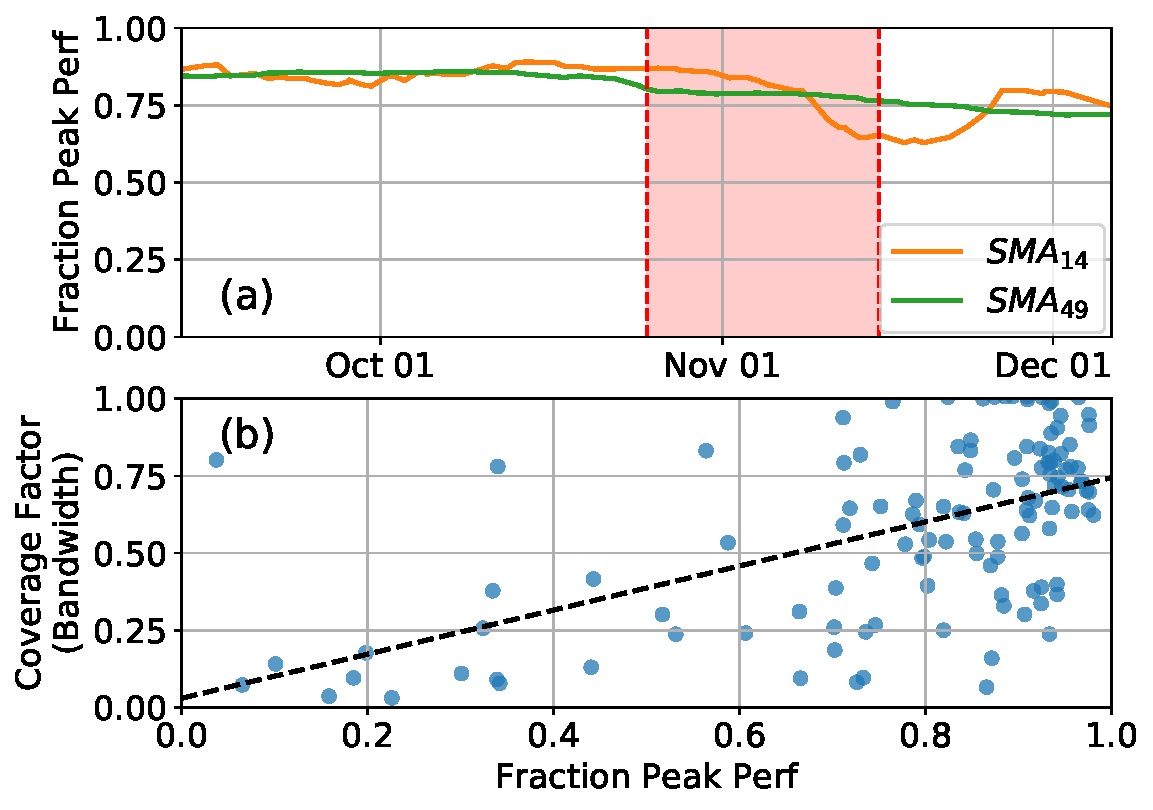
\includegraphics[width=1.0\columnwidth]{mira-correlation-region}
    \vspace{-.35in}
    \caption{Correlation between performance and $CF_{bw}$ in a divergence region on \mira for all I/O motifs combined.
    (a) highlights the divergence region of interest and corresponds to the same highlighted region shown in Fig. \ref{fig:mira-regions-overview}. (b) shows the correlation between performance and $CF_{bw}$ in that region.
    Correlation coefficient is $0.507$ and p-value is ${8.71 \times 10^{-9}}$; dashed line in (b) is a linear fit with slope $0.503$ drawn for visual aid.}
    \label{fig:mira-correlation-region}
    % source: sc18_region-correlation.ipynb
\end{figure}

% Bandwidth, IOPS, and metadata contention are confidently correlated with I/O performance at both long. 

\TODO{add a footnote explaining p-value}
We begin our correlative analysis by partitioning a year-long data set into
divergence regions using the method described in
Section~\ref{sec:features/partitioning}.  Using observations from \mira
\mirafsone as an example, we set ${w_{short} = \textup{two weeks}}$ and ${w_{long}
= \textup{seven weeks}}$ to identify divergence regions, and then discard any
regions with fewer than three data points.  Regions with few data points are discarded
for two reasons: (a) intuitively, very short divergence regions occur
when $\textup{SMA}_{short} \approx \textup{SMA}_{long}$ and there is
minimal long-term variation, and (b) statistically, it is impossible
to assert the statistical significance of a correlation with fewer than
three data points.  This yields 32 divergence regions.

We then apply Pearson correlation~\cite{Falk97manyfaces} to the feature vectors within each divergence region to identify the factors that correlate with its
performance trend.
The result of this process is a new feature vector for each divergence region which contains the correlation coefficients between the fraction of peak performance and every other attribute across all observations in that region.
We then use the p-value of each correlation coefficient\footnote{
The p-value of a correlation coefficient is the probability of observing data that would show the same correlation coefficient in the absence of any real relationship between the underlying metrics.
A low p-value indicates that it is extremely unlikely that the calculated correlation coefficient would be observed if the metrics being compared had no real correlation.
As such, p-values represent the statistical significance of a statistical measurement.}
to further downselect the total set of regions to those with extremely high significance
($\textup{p-value} < {1.0 \times 10^{-5}}$).
This threshold yields a total of nine relevant divergence regions on \mira \mirafsone which are all depicted as shaded extents in Figure \ref{fig:mira-regions-overview}.
Each of these nine regions exhibits at least moderate correlation ($R$) ranging from 0.507 to 0.884 with the bandwidth coverage factor feature.

\TODO{I'm not sure I understand why we're aggregating divergence regions from different motifs here, since everywhere else our analysis is applied to these independently. For one, different motifs could have different trend regions by definition. If the results hold over just one motif, maybe just use those, or something? -SS}
Fig.~\ref{fig:mira-correlation-region} illustrates the correlation between bandwidth coverage factor and fraction peak performance for a particular divergence region in November 2017 on \mira \mirafsone.
This example exhibits the lowest correlation ($R = 0.507$) with bandwidth coverage factor of any of the selected regions, and the scatter plot of performance results shows why:
this region contains a cluster of poorly performing probes (${0.2 < \textup{fraction peak perf} < 0.4}$) that ran with a relatively high bandwidth coverage factor.
This region is also the single largest divergence region observed on \mira; a difference of over 20\% between $\textup{SMA}_{short}$ and $\textup{SMA}_{long}$ was observed during this time.
This divergence region example highlights the importance of not just identifying regions and calculating correlations, but identifying cases in which the analysis indicates the presence of an unknown factor that is not adequately captured by the instrumentation framework.

Despite the unusual region shown in Fig. \ref{fig:mira-correlation-region},
however, these data indicate that the time-dependent performance divergences observed on \mira show either moderate or strong correlation with bandwidth contention.
Additionally, this correlation with performance degradation occurs across
\emph{all} I/O motifs (similar to Figure \ref{fig:regions-heatmap}a) which
distinguishes it from the motif-specific case discussed in Section
\ref{sec:features/timedependent}.  

When the same Pearson correlation is calculated across the entire collection
of \mira \mirafsone data in the absence of partitioning, the correlation with bandwidth coverage factor
yields an overall result of $R = 0.483$ and $\textup{p-value} =
2.25\times 10^{-88}$.  \textbf{Thus, significantly stronger
correlations can be found by focusing analysis on algorithmically identified regions of
interest in the data.}

% \TODO{We could use a plot for comparison if we have a lot of free time to
% kill.  I don't think it is critical though.}

\subsection{Survey of divergence regions} \label{sec:results/correlate-all}

% - Bandwidth, IOPS, and metadata contention are confidently correlated with I/O performance at both long. 



\begin{figure}
    \centering
    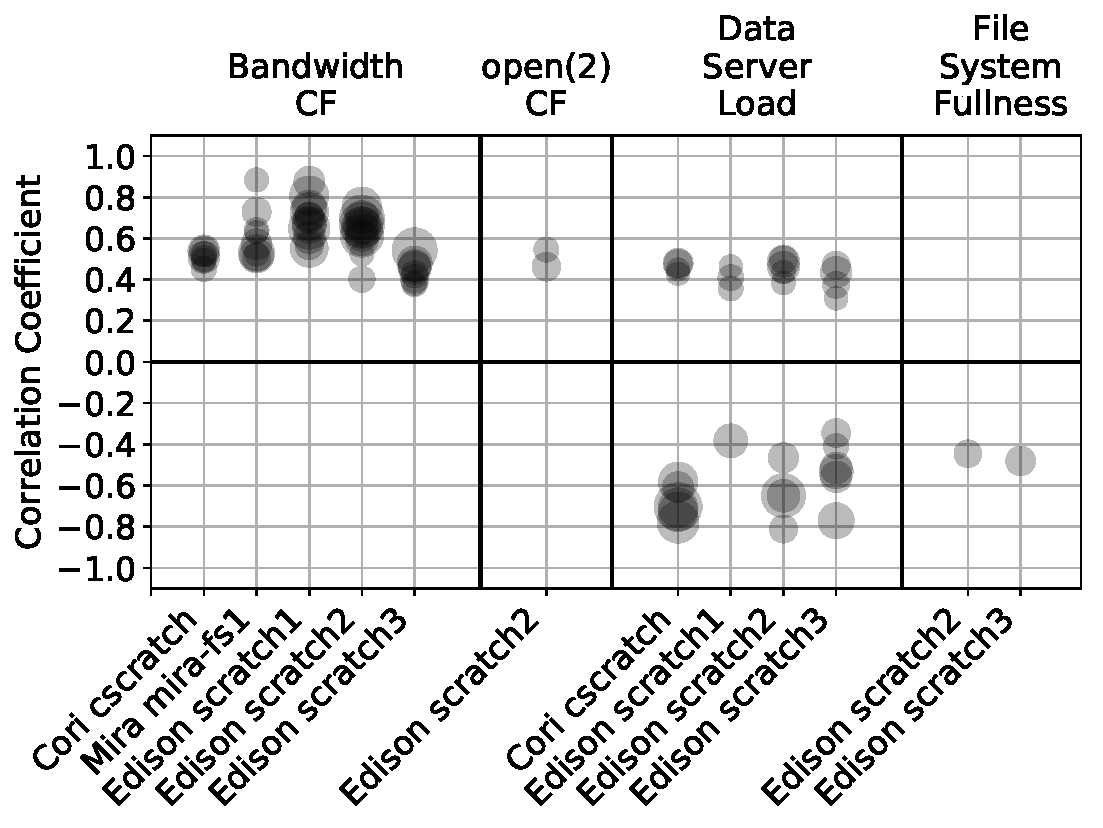
\includegraphics[width=1.0\columnwidth]{trend-correlations}
    \vspace{-.35in}
    \caption{Correlations discovered between fraction peak performance and all other attributes measured during job execution.
    Each circle represents the correlation coefficient over a single trend region, and its diameter is proportional to $-\log_{10}(\textup{p-value}$).
    CF denotes coverage factor.}
    \label{fig:trend-correlations}
    % source: sc18_region-correlation-all.ipynb
\end{figure}



Next we apply the same correlation analysis to the other test platforms in our study, again only keeping correlations with an extremely high significance ($\textup{p-value} < {1.0 \times 10^{-5}}$), and the results of this analysis are shown in Fig. \ref{fig:trend-correlations}.
As was found with Mira in Section \ref{sec:results/correlate-mira}, there is moderate to strong correlation between I/O performance and the bandwidth coverage factor on the Lustre file systems of \cori and \edison.
Although bandwidth contention resulting in performance loss is intuitive at the scale of a single performance transient, the fact that these correlations were found over longer-term divergence regions indicates that \textbf{bandwidth contention from \emph{sustained workloads} often accompanies sustained performance losses}.
This is particularly relevant to the increasing fraction of experimental and observational data that is being processed on modern HPC platforms; as the volume of data being continually streamed from large-scale scientific instruments increases, the effects of sustained bandwidth contention are likely to become increasingly prominent.

% - The sign and magnitude of the correlations changes over time.

\begin{figure}
    \centering
    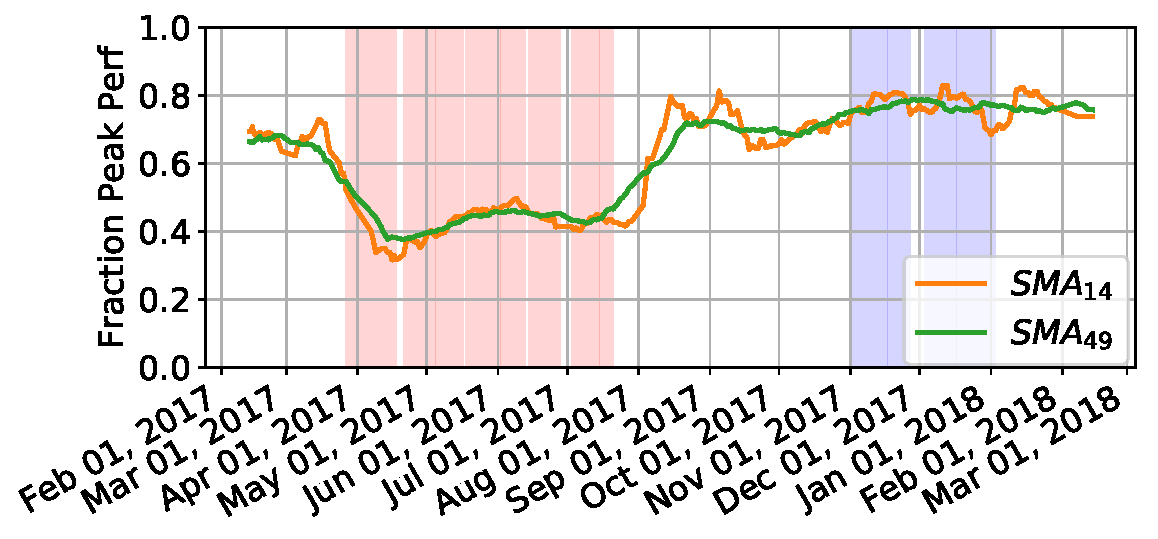
\includegraphics[width=1.0\columnwidth]{cscratch-bimodal-fsaveosscpu}
    \vspace{-.35in}
    \caption{Regions of negative correlation (red) and positive correlation (blue) between fraction peak performance and data server load during trend regions identified on \cori.
    SMAs for \cori's HACC write workload also shown to illustrate the coincidence of a long-term performance issue with the direction of correlation.}
    \label{fig:cscratch-bimodal-fsaveosscpu}
    % source: sc18_region-correlation-all.ipynb
\end{figure}


Another noteworthy feature that this method reveals is the bimodality of correlation between performance and the CPU load of the file system data servers (``Data Server Load'' in Fig. \ref{fig:trend-correlations}) on the Lustre-based test platforms.
A time-resolved view of the regions where performance correlates with data server CPU loads (Fig. \ref{fig:cscratch-bimodal-fsaveosscpu}) reveals that the bimodality of the correlation matches the biomodality observed in the HACC write workload on the affected storage systems.
During the long-term performance regression discussed in Section \ref{sec:features/timedependent}, high CPU load on the Lustre OSSs coincided with low performance of the I/O performance probes.
As soon as performance was restored on August 10, the relationship reversed, and high CPU load was observed favorably with respect to performance.

The positive correlation between performance and CPU load is consistent with the data servers using CPUs primarily to service incoming I/O requests, whereas the negative correlation indicates that another CPU load (as may be caused by an algorithmic bug) was present and competed with the data servers' ability to use CPU to service those same requests.
From this, we conclude that not only does baseline I/O performance vary with time, but \textbf{the nature and magnitude of how different attributes correlate with I/O performance also change over time}.
Had this correlation analysis been performed without partitioning over divergence regions, the regions of positive and negative correlation would have obfuscated each other in the net result.

The remaining two attributes that were found to correlate with performance
are file system fullness and \texttt{open(2)} coverage factor (a
measure of metadata resource contention).  The two instances of file
system fullness correlating negatively with performance are clear
and can be corroborated with independent observations from facilities
staff.  These two regions encapsulate periods when their respective
file systems approached 90\% fullness for a period of several days.
The observed loss of performance is consistent with Lustre's known
susceptibility to significant performance degradation as OSTs approach
90\% fullness~\cite{oral2014best,Lockwood2017}.

The correlation with
\texttt{open(2)} coverage factor is intuitive because this metric acts as a
proxy for metadata contention.  
One of these divergence regions was found to overlap with an unusually extensive, long-running multi-day purge of the \edison \scratchtwo file system.
However, it is unclear at this time what caused the other correlated divergence region.
% The above statement is not very satisfying, but we don't have time to do more detailed analysis.  The regions are:
% coverage_factor_opens 2017-03-29 19:11:51 - 2017-04-15 19:13:37 (71 points)
% coverage_factor_opens 2017-11-26 18:26:41 - 2017-12-13 20:03:11 (141 points)


\subsection{Transient performance loss} \label{sec:results/shortterm}

\begin{figure}

    \centering
    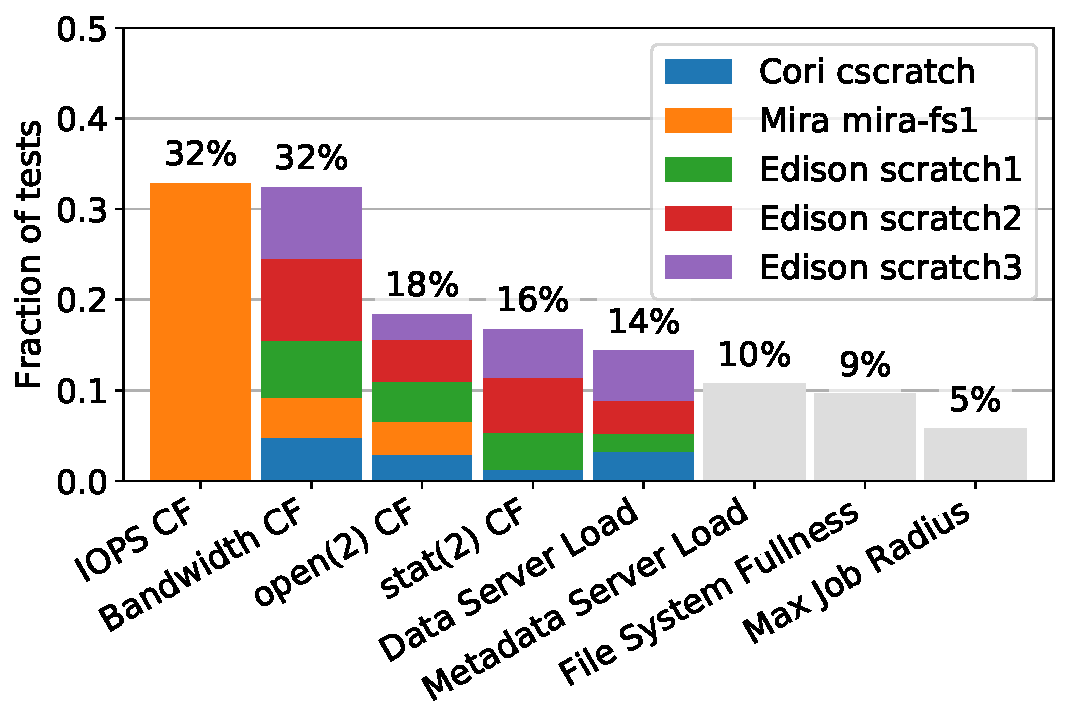
\includegraphics[width=1.0\columnwidth]{contributors-bad-by-system-grey}
    \vspace{-.35in}
    \caption{Attributes that correlated with poor I/O performance across all file systems and benchmarks tested normalized to the number of probes during which each attribute was measured.
    \mira was the only system for which IOPS coverage factor was measured.
    Greyed bars are attributes whose aggregate contributions were not statistically significant.
    Percentages do not add up to 100\% because multiple attributes are often classified as contributors for a single anomalous observation.
    }
    \label{fig:contributors-bad-by-system}
    % source: sc18_umamify-all.ipynb
\end{figure}

In addition to characterizing long-term performance issues, it is also advantageous to determine the reasons why I/O performance is severely degraded for one and only one day in an otherwise unremarkable period of time.
Such performance losses, exemplified as isolated dark blocks in Fig. \ref{fig:regions-heatmap}, may only be observed in one of the I/O performance probes issued on that day, suggesting a very short-lived issue that disappeared over the course of one or two of the eight daily probes.
The lack of a consistent performance trend surrounding these transients makes them difficult to correlate with other metrics as was done in the previous section, necessitating a different approach to characterizing them.

To address this need, we apply the same strategy of partitioning performance observations into divergence regions and then performing statistical analysis within each region.
To identify individual performance anomalies in a divergence region and classify the factors which contributed to them, we apply the following binary classification method:
\TODO{Are we sure we only want to determine one and only one anomalous observation in each divergence region? -SS}

\begin{enumerate}[leftmargin=*]

\item We examine the feature vector for every observation in the divergence region, and for each attribute $a$, determine the observation where that attribute's measured value was at its lowest, $\min(a)$.

\item We then define the \emph{anomalous observation} for the divergence region as the observation whose feature vector contains $\min(a)$ for fraction peak performance.
As divergence regions contain observations of similar performance by definition, this anomalous observation is truly anomalous-- it is differentiated from the long-term performance trends described in Sec.~\ref{sec:features} as well as the ones within its own divergence region.

\item Finally, we determine which other $\min(a)$ values also fall in this anomalous observation's feature vector and classify those attributes as contributors to the anomalous observation's performance.

\end{enumerate}

Qualitatively, this process codifies the conjecture that if I/O performance is anomalous on a specific day, the other measured attributes which were also anomalous at that time are what contributed to that behavior.
Quantitatively, this simple classification scheme allows us to identify relationships and define the statistical significance of each classification for individual anomalous observations using p-values\footnote{
The p-value is the probability of making a positive classification in the absence of an underlying relationship or, equivalently, the probability of positively classifying a random value.
Since there is only one $\min(a)$ in each region of $N$ observations, the p-value for our classifications is thus $\frac{1}{N}.$}.

The result of this process is zero or more attributes being positively classified as contributors to anomalous performance.
For example, if the lowest values of the bandwidth coverage factor and IOPS coverage factor attributes occur in the same feature vector as the lowest value for performance, we classify both bandwidth and IOPS coverage factors as contributors to that anomalous observation's performance.

To apply this method, we first group observations into sets of data by the test platform on which they ran as was done in Section \ref{sec:results/correlate-mira}.
These sets are then further subdivided according to I/O motif and read/write mode of the probe to classify anomalies at full temporal resolution and motif-level granularity.
The net result are $5 \times 4 \times 2 = 40$ sets of data, each representing a unique combination of test platform ($5 \times$, as listed in Table \ref{tab:platform-descriptions}), I/O motif ($4 \times$, per Table \ref{tab:benchmark-motifs}), and whether the probe was reading or writing ($2 \times$).
Schematically, each horizontal row in Figure \ref{fig:summary-heatmap} represents a single set.
For each set of observations, SMAs are calculated, crossover points are defined, and the set is partitioned into a set of divergence regions.

This partitioning results in 1,146 divergence regions across 40 sets of observations, each containing one anomalous observation.
For each divergence region, we then apply the aforementioned binary classification to generate positive classifications of attributes that affected performance and their p-values.
We discard all statistically insignificant classifications ($\textup{p-value} > 0.10$) to eliminate divergence regions that are too small to make any meaningful classifications, positive or negative.
The final products are 490 anomalous observations, 410 of which have at least one attribute positively classified as a contributor.

As described in Section \ref{sec:methods/tokio}, not every observation's feature vector has every feature defined.
So as not to bias our results away from those attributes that were only measured for a subset of observations (e.g., IOPS coverage factor was only collected on \mira), we calculate the frequency of each attribute as the ratio of observations where it was defined \emph{and} classified to the number of observations where it was defined.
The result of this aggregate frequency summary is shown in Figure \ref{fig:contributors-bad-by-system}.
\TODO{Glenn to clean up above paragraph}

As with the longer-term performance divergence characterized in Section \ref{sec:results/correlate-all}, high contention for bandwidth is found to also coincide with short-term performance transients.
However, contention for IOPS is also positively classified in a significant fraction of anomalous observations despite it not arising as a factor in longer-term performance divergence.
This contrast demonstrates that IOPS contention only becomes a statistically significant attribute related to performance degradation in short-term transients, and there are no sustained periods of high IOPS on \mirafsone.
This also distinguishes this utility of this transient classification from
the longer-term correlative analysis.
% Intuitively this result makes sense, as a job running on the machine performing I/O only places load on the metadata server during short duration events (eg. file open/close), whereas the load when the data is being read or written is likely to occur over much longer time periods.
% Intuitively, this result makes sense; a job performing I/O nominally places load on the metadata server only at the start and end of of reading and writing, while the process of reading and writing occurs over much longer time periods.
% \TODO{gkl: Phil/Shane, please review above line with your I/O expert hat on}

We also observe the coincidence of anomalous jobs and anomalous metadata coverage factor and CPU load on
data servers to a less significant degree.  This is
consistent with the moderate correlations shown in
Figure~\ref{fig:trend-correlations}.
Unlike the correlative analysis, however, metadata contention was found to impact individual jobs on every test platform and occurred at much higher frequency.
These findings indicate that metadata contention is much more likely to coincide with transient performance loss than a long-term and sustained divergence of performance.

In general, the contrast in correlations between transient events and
long-term trends shows that \textbf{the attributes that correlate with transient
performance problems (IOPS and
  metadata contention) often differ from those that correlate with
    long-term performance problems (bandwidth contention).} These are two distinct forms of performance variation that
require unique investigation techniques.

\TODO{Simplify our motivation for doing this bimodal stuff--we saw some metrics that correlated infrequently.  Are these statistically significant?
\\
"frequency of attributes" should go away--we're talking about how often $a$ pops up in "instance of slowdowns"
}
Metadata server CPU load, file system fullness, and maximum job radius were also classified in some anomalous observations.
However, the low number of anomalous observations in which they appeared calls into question the statistical significance of these three findings.
To address this, we calculate the p-values, or the probability of observing the same number of classifications in the absence of a true underlying relationship, for each metric\footnote{
To calculate these p-values, we use one-tailed binomial tests using the number of positive classifications observed for each metric.
The fact that our dataset was filtered to only include regions with ${\textup{p-value} < 0.10}$ also establishes 0.10 as the most conservative value for the binomial test probability.}.

The result of these significance tests reveal that the number of times metadata server load, file system fullness, and maximum job radius were classified is statistically insignificant.
Whereas the leftmost five attributes in Fig. \ref{fig:contributors-bad-by-system} all have p-values of ${5 \times 10^{-5}}$ or lower, the insignificant metrics' are 0.15 or higher.
Qualitatively, these negative findings are not unreasonable; for example, file system fullness is most often a degenerative, long-term health problem as was identified in Section \ref{sec:results/correlate-all} and prior work~\cite{oral2014best,Lockwood2017}.

The classification process and analysis described here demonstrates that it is possible to apply statistical analysis to fine-grained divergence regions and still obtain statistically significant insight into the causes of transient performance degradation.
While we chose a very simple binary classification criteria based on $\min{a}$, this process could be applied using any classification methodology that identifies relationships between feature vectors in a divergence region and quantifies the associated statistical significance.


\endinput

% NJW - this sentence adds too much complexity to end the section with
% 
%%%For example, classifying attributes based on quartiles rather than minima would be feasible with more coarse-grained divergence regions to offset the decrease in significance inherent in the selection criteria.

\subsection {Discussion}
\label{sec:results/discussion}

\TODO{This is where interesting dribs and drabs are winding up.  Do we carve out a separate section about this stuff, or just drop it?}

Our choice of averaging $\textup{SMA}_{short}$ over ${-0.5w_{short} <= t < +0.5w_{short}}$ makes it insensitive to choice of $w_{short}$.
For the analysis in Section \ref{sec:features/timedependent} changing $\textup{SMA}_{short}$ from $\textup{w}_{14}$ to both $\textup{w}_{7}$ and $\textup{w}_{28}$ resulted in no change to the dates bounding the 139-day divergence region.
The principal effect of changing $\textup{w}_{short}$ is the number of short regions that arise from the higher-frequency oscillations of $\textup{SMA}_{short}$ around $\textup{SMA}_{long}$.

\TODO{This is where a discussion about performance models having to account for long-term changes to baseline performance should go.  That doesn't seem to fit well into the rest of the narrative though.}

We found the exact choice of $w_{short}$ and $w_{long}$ to be somewhat arbitrary; adjusting these values by as much as $\pm 50\%$ did not affect the identification of the most significant events presented here.
In addition, a specific choice of $w$ does not preclude analyzing events longer or shorter than $w$, and we demonstrate methods to address this in Sections XYZ.

Although SMA crossover points are also applied in market analysis for detecting trends in prices and predicting when to buy or sell an asset based on the direction of the crossover~\cite{brock1992simple}.
However, the predictive value of SMA crossovers is a source of controversy even in the financial community, and thus, we focus here solely on using them as tools for detecting trends and partitioning divergent regions in historical datasets.

Financial market analysis techniques can be used to detect underlying trends within noisy I/O performance data.


% \section{Conclusion} \label{sec:conclusions}

Our study of a year in the life of a parallel file system provided a
variety of insights into performance variation on production systems,
including both long-term trends and transient anomalies.  These insights,
and the methods that we used to derive them, have implications for
instrumentation methods, administrative expectations, and analysis
techniques. Some of the recommendations in these findings can be acted on
now by broadening the scope of instrumentation or enhancing analysis tools based on observations in this paper.
Others more fundamentally motivate the need for ``live'' analysis of
production systems so that the lessons learned here (especially those
related to dynamic, time-dependent behavior) can be more generally extracted
at any time from a running system to produce actionable feedback.

Near term future work calls for the development of additional \tokio
connectors to incorporate additional storage resources such as burst
bufferss.
In the long term, we plan to develop methods to systematically classify the
similarity of different regions from one another and enable the
determination of broad classes of performance regions.
We will also use the measured data as input for simulation frameworks to
enable the design of potential new file system features or policies that may
reduce the amount of I/O performance variation seen in production. 
\endinput

\begin{enumerate}

\TODO{these lack "implications for state of the practice"; need to take these up a level.  if we were selling this process to another center, what would they need to take from this study?}

\item \textbf{Baseline performance and performance variation changes over time.}
We have shown that the baseline peak performance for a given I/O motif on a file systems can change over time as a result of factors such as system software updates and sustained workloads motivated by external factors such as end of allocation year.
\TODO{1. you can't just measure performance on day 1}

\item \textbf{The magnitude and sign of correlation between performance and other measured metrics also varies over time.} 
We demonstrated that high CPU load can correlate with favorable performance under healthy file system conditions, and it can coincide with unfavorable performance when non-I/O workloads are impacting storage servers.
\TODO{2. be careful how you interpret your metrics; training a model on one dataset might not make it apply to others}

\item \textbf{Bandwidth, IOPS, and metadata contention are often confidently correlated with I/O performance problems are occurring.}
We were able to obtain statistically significant trends about isolated performance transients by aggregating simple binary classifications based on coincident observations of worst values within regions.
That said, some jobs defied classification using our binary classification method.
This indicates that we are still missing telemetry from important components of the I/O subsystem that contribute to performance variation.
\TODO{3. metadata contention is burstier than bandwidth, but they both affect performance.  just at different time scales}

\item The methods presented here are not dependent on SMAs, and alternative approaches for both partitioning time series data and classifying the measurements within regions can be replaced with more sophisticated methods.
What we have shown is that a great deal of information about I/O performance variation can be quantified using holistic I/O analysis and simple statistical methods.
\end{enumerate}


% % use section* for acknowledgment
\section*{Acknowledgments}

The authors would like to thank...

% trigger a \newpage just before the given reference
% number - used to balance the columns on the last page
% adjust value as needed - may need to be readjusted if
% the document is modified later
%\IEEEtriggeratref{8}
% The "triggered" command can be changed if desired:
%\IEEEtriggercmd{\enlargethispage{-5in}}

% references section

% can use a bibliography generated by BibTeX as a .bbl file
% BibTeX documentation can be easily obtained at:
% http://www.ctan.org/tex-archive/biblio/bibtex/contrib/doc/
% The IEEEtran BibTeX style support page is at:
% http://www.michaelshell.org/tex/ieeetran/bibtex/
\bibliographystyle{IEEEtran}
% argument is your BibTeX string definitions and bibliography database(s)
\bibliography{IEEEabrv,references}
%
% <OR> manually copy in the resultant .bbl file
% set second argument of \begin to the number of references
% (used to reserve space for the reference number labels box)
%\begin{thebibliography}{1}
%
%\bibitem{IEEEhowto:kopka}
%H.~Kopka and P.~W. Daly, \emph{A Guide to \LaTeX}, 3rd~ed.\hskip 1em plus
%  0.5em minus 0.4em\relax Harlow, England: Addison-Wesley, 1999.
%
%\end{thebibliography}




% that's all folks
\end{document}